\documentclass{article}
\usepackage[UTF8]{ctex}  % 使用中文支持包
\usepackage[a4paper, margin=1in]{geometry}  % 设置纸张大小和边距
\usepackage{anyfontsize}  % 解决字体大小报错问题
\usepackage{fancyhdr}  % 设置页眉、页脚、页码
\usepackage{lscape}
\usepackage{longtable}  % 支持长表格
\usepackage{booktabs}
\usepackage{graphicx}
\usepackage{colortbl}
\usepackage{tabularx}
\usepackage{multirow}
\usepackage[table,xcdraw]{xcolor}

\usepackage{amsmath}  % 数学公式支持
\usepackage{cases}  % 支持联立编号
\usepackage[sort]{natbib}  %国标参考文献 with sorting option

\usepackage{graphicx}  % 插入图片支持
\usepackage{float}  % 设置图片浮动位置
\usepackage{subfigure}  % 插入多图时用子图显示

\usepackage{listings}  % 代码块支持
\usepackage{xcolor}  % 设置代码块颜色

\lstset{
    basicstyle          =   \sffamily,          % 基本代码风格
    keywordstyle        =   \bfseries,          % 关键字风格
    commentstyle        =   \rmfamily\itshape,  % 注释的风格,斜体
    stringstyle         =   \ttfamily,  % 字符串风格
    flexiblecolumns,                % 别问为什么,加上这个
    numbers             =   left,   % 行号的位置在左边
    showspaces          =   false,  % 是否显示空格,显示了有点乱,所以不现实了
    numberstyle         =   \zihao{-5}\ttfamily,    % 行号的样式,小五号,tt等宽字体
    showstringspaces    =   false,
    captionpos          =   t,      % 这段代码的名字所呈现的位置,t指的是top上面
    frame               =   lrtb,   % 显示边框
}

\lstdefinestyle{Python}{
    language        =   Python, % 语言选Python
    basicstyle      =   \zihao{-5}\ttfamily,
    numberstyle     =   \zihao{-5}\ttfamily,
    keywordstyle    =   \color{blue},
    keywordstyle    =   [2] \color{teal},
    stringstyle     =   \color{magenta},
    commentstyle    =   \color{red}\ttfamily,
    breaklines      =   true,   % 自动换行,建议不要写太长的行
    columns         =   fixed,  % 如果不加这一句,字间距就不固定,很丑,必须加
    basewidth       =   0.5em,
}

\usepackage[hyphens]{url}  % 支持链接换行
\usepackage{hyperref}  % 超链接支持

\hypersetup{
    hidelinks,
    colorlinks=true,
    allcolors=black,
	pdfstartview=Fit,
	breaklinks=true
}

\usepackage{gbt7714}  %国标参考文献

\bibliographystyle{gbt7714-numerical}

\usepackage{lastpage}  % 添加lastpage包

\newcommand\f[2]{\frac{#1}{#2}}
\newcommand\pf[2]{\frac{\partial#1}{\partial#2}}
\newcommand\df[2]{\dfrac{#1}{#2}}
\newcommand\pdf[2]{\dfrac{\partial#1}{\partial#2}}
\newcommand\zsin[1]{\frac{e^{i#1}-e^{-i#1}}{2i}}
\newcommand\zdsin[1]{\dfrac{e^{i#1}-e^{-i#1}}{2i}}
\newcommand\zcos[1]{\frac{e^{i#1}+e^{-i#1}}{2i}}
\newcommand\zdcos[1]{\dfrac{e^{i#1}+e^{-i#1}}{2i}}
\newcommand\zline[1]{#1-\overline{#1}}
\newcommand\dg[2]{#1^{\circ}#2'}

\setlength{\headheight}{16pt}
\pagestyle{fancy}
\fancyhf{}

\title{\bf\huge 压力容器内部中子的产生、输运、控制}
\author{Jerry}
\date{\today}
\pagenumbering{arabic}

\begin{document}

\fancyhead[L]{Jerry}
\fancyhead[C]{压力容器内部中子的产生、输运、控制}
\fancyhead[R]{核电厂系统与设备-黄善仿}
\fancyfoot[C]{\thepage}

\maketitle

\section*{摘要}

这篇文章概述了压水堆中中子的产生、输运和控制机制,以及堆芯燃料和控制棒的设计方法。压水堆中,中子主要通过铀-235或钚-239的裂变产生,并通过链式反应持续释放能量。中子的输运由中子与介质的碰撞决定,可用中子输运方程描述。反应性控制方式包括控制棒、可燃毒物和硼酸等。这些方法通过改变中子吸收、慢化能力或燃料含量来调节反应堆的反应性,压水堆一般结合使用以减少控制棒数量。堆芯燃料设计涉及燃料材料、形状、排列等因素。优化燃料装载配置能够提高能量输出和反应堆安全性。控制棒设计注重材料选择,以银-铟-镉或铪合金为主,通过复合材料改进并配备水压驱动系统,实现有效控制。

\subsubsection*{关键词: 1. 压水堆; 2. 核反应堆; 3. 堆芯; 4. 核能; 5. 热工水力}

\section{引言}

在核能领域,压水堆(PWR)作为当前最常见的反应堆类型之一,广泛应用于核电站中,用于安全高效地发电。压水堆的工作原理基于铀-235或钚-239的裂变反应,通过中子的引发和持续释放,形成链式反应并产生能量。然而,为了确保反应堆的稳定运行,中子的输运与反应性控制显得尤为重要。这不仅关系到反应堆的功率输出,还涉及核燃料的使用效率和设备的长期安全性。

本篇文章主要探讨了压水堆内中子的产生、输运和控制方法,进一步分析了堆芯燃料和控制棒的设计对反应堆性能的影响。文章在阐述中子在反应堆中的运动和控制原理的基础上,着重介绍了堆芯燃料的排列优化、燃料组件设计改进以及控制棒材料的选择与驱动系统设计。通过这些设计与控制手段的优化,不仅能提升反应堆的安全性和经济性,还能在最大限度内提高核燃料的利用率和反应堆的使用寿命。

\section{中子的产生、输运、控制原理}

\subsection{中子产生}
在压水堆中,中子主要来源于铀-235(U-235)或钚-239(Pu-239)的核裂变反应。当这些重核吸收一个中子后,它们会变得不稳定并分裂成两个较轻的核,同时释放出额外的中子和能量。这些释放出的中子可以继续引发其他重核的裂变,从而形成一个链式反应。链式反应的持续进行是压水堆产生能量的基础。

\subsection{中子输运}
通常,在反应堆内中子数密度比介质的原子数密度要小得多,因此中子在介质内的运动主要是中子和介质原子核的碰撞结果,而中子之间的相互碰撞可以忽略不计。原来在某一位置具有某一能量和运动方向的中子,经过一段时间后,将以不同的能量和运动方向出现在另一位置。这种现象称为中子输运。中子输运方程为式\ref{eq:neutron_transport}。

\begin{equation}
    \begin{aligned}
        \pf{\phi/v(E)}{t} & + \vec{\Omega} \cdot \nabla \phi + \Sigma_t(\vec{r}, E) \phi = \\
                          & \int_{0}^{\infty}\left[\int_{\vec{\Omega}'}\Sigma_s(\vec{r}, E') f(\vec{r}, E'\rightarrow E, \vec{\Omega}'\rightarrow\vec{\Omega})\phi(\vec{r}, E', \vec{\Omega}', t)d\vec{\Omega}'\right]dE' \\
                          & + \frac{\chi(E)}{4\pi}\int_{0}^{\infty}\left[\int_{\vec{\Omega}'}\nu(E')\Sigma_f(\vec{r}, E')\phi(\vec{r}, E', \vec{\Omega}', t)d\vec{\Omega}'\right]dE' \\
                          & + S(\vec{r}, E, \vec{\Omega}, t)
    \end{aligned}
    \label{eq:neutron_transport}
\end{equation}

\subsection{中子控制}

凡是能够有效地影响反应性的任何装置、机构和过程都可以用作反应性的控制。归纳起来有下列3种方法:

\begin{itemize}
    \item 改变堆内中子吸收。在堆芯中加入或提出控制材料以改变堆内中子的吸收。目前广泛采用的控制材料有可移动式控制棒、固体可燃毒物棒和在液体冷却剂中加入可溶性毒物(如硼酸)。
    \item 改变中子慢化性能。例如在谱移反应堆中(重水-轻水混合慢化反应堆),通过改变重水与轻水的比例,以改变中子能谱,从而改变反应性。
    \item 改变燃料的含量。在用燃料来作控制棒或作控制棒跟随体的情况下,当控制棒移动时,除了改变堆内中子吸收之外,还可改变堆内燃料量,从而改变反应性。改变中子泄漏。在小型快中子反应堆中,可用移动反射层的方法,改变中子的泄漏, 从而改变反应性。
\end{itemize}

选择哪种控制方式是与堆型有关的。目前压水反应堆采用的反应性控制方式主要有如下3种:1)控制棒控制;2)固体可燃毒物控制,主要用于补偿部分初始过剩反应性;3)化学补偿控制,主要是在冷却剂中加入可溶性硼酸溶液来补偿过剩的反应性。

在轻水反应堆中,初始剩余反应性很大,控制棒的效率又比较低,如全部都采用控制棒来控制,则需要控制棒的数目就很多。而轻水反应堆的栅格较稠密,反应堆体积较小,安排这么多的控制棒是有困难的,同时也使压力顶盖开孔增加,影响压力容器的强度。所以,目前在压水反应堆中,都是采用控制棒、固体可燃毒物和冷却剂中加硼酸溶液三种控制方式来联合控制,以减少控制棒的数目。

\section{堆芯燃料设计}
堆芯燃料棒的设计与固体可燃毒物主要影响中子的产生与输运。堆芯燃料棒的设计主要包括燃料的选择、燃料的几何形状、燃料的分布等。

堆芯燃料管理涉及堆芯中数百个燃料组件的最佳排列。从经济角度来看,这种排列的优化对于提高核电站的竞争力非常重要。最佳核燃料重新装载设计可以定义为在满足安全约束(如峰值功率因数限制)的前提下,在给定的燃料库存下具有最大循环长度的配置,或者在给定的循环长度下使用最少量的可裂变材料。

燃料组件位置确定的主要问题是堆芯燃料装载模式可能存在大量组合。此外,由于这是一个非线性和离散问题,使用传统优化技术会变得复杂。为了优化堆芯燃料组件的分布,人们开发了几种技术。在燃料组件装载配置方面,更好的选择对于保证裂变元素的充分利用以及运行过程中的安全至关重要。

燃料组件主要由下管座、上管座、燃料棒、导向管以及定位格架组成。以AP1000为例,AP1000燃料组件是基于RFA-2组件和RFA-2(XL)组件改进而成的。RFA-2燃料组件的活性区长度为12英尺,在靠近顶部的中间格架之间设置了三层搅混格架。RFA-2(XL)组件的活性区长度为14英尺,未设置搅混格架。AP1000燃料组件采用14英尺的活性区长度,在高热流密度区域,增设4层搅混格架。并对燃料组件加以改进,包括抬高了活性区,降低堆芯下板注量,延长RV寿命;降低管座高度,降压降;燃料棒增加下气腔设计;增大燃料棒与上管座之间间隙,提供更多燃料棒生长空间等。\cite{HanXiangZhenDiSanDaiFanYingDuiAP1000HeEPRDeDuiXinHeSheJi2013}

考虑了多种不同的装载模式,得出的总体结论是,当堆芯中的功率分布尽可能平坦时,从燃料中提取的能量就越多。优化装载模式的常用方法包括高度工程判断、一套启发式规则、一种优化算法以及用于评估所提装载模式的计算机代码。

对于燃料棒的排列,AP1000燃料组件呈17×17方阵排列,包含264根燃料棒,24根控制棒导向管,1根中央测量管。燃料芯块由稍加富集的UO2粉末经冷压后烧结而成,两端为浅碟型,并在两端外圆柱面上留有倒角。燃料包壳为ZIRLO合金。AP1000燃料组件的格架包括10层结构格架(顶部格架、底部格架、8层中间格架)、4层中间搅混格架以及1层保护格架。其中,顶部和底部格架的材料为INCONEL,中间格架和中间搅混格架的材料为ZIRLO合金。ZIRLO合金具备较低中子吸收截面,有良好的中子经济性能;较高的抗冷却剂、燃料和裂变产物腐蚀能力;更好的抗辐照生长和蠕变的性能,在运行温度下有高机械强度和延展性。有利于加深燃料的燃耗。INCONEL合金具有丰富的压水堆使用经验,可确保满足反应堆运行对材料的要求。\cite{HanXiangZhenDiSanDaiFanYingDuiAP1000HeEPRDeDuiXinHeSheJi2013},可以看出,在棒状的燃料中,燃料的材料、几何形状、分布等都会影响中子的输运,且应该根据具体的堆芯设计来进行优化。

对于燃料材料的选择,一般采用1.8\%~5.0\%富集度的UO2燃料,并按照不同的浓度进行组装\cite{JiSongTaoXiaoXingFanYingDuiHuanXingRanLiaoZuJianSheJiJiYingYongYanJiu2023}。大多数情况下,浓缩度高的燃料位于内侧,而浓缩度低的燃料位于四角。\cite{LiuGuoMingHPR1000DuiXinZhuangZai50MOXZuJianDeRanLiaoGuanLiFangAn2017}\cite{muratResearchAP1000Fuel2021}

除了圆柱形燃料之外,还有一些新型燃料设计,如螺旋十字形燃料等,通过改进燃料的设计,可以较大的提升反应堆的热工水力性能。

螺旋十字形燃料最早被Conboy于约2007年设计\cite{conboyThermalHydraulicAnalysisCrossShaped},并计算了其热工水力性能\cite{conboyEvaluationHelicalCruciformFuel2014}。参考熊敏智的论文,螺旋十字形燃料的设计如图\ref{fig:cross_shaped_fuel}所示\cite{XiongMinZhiJiYuMengTeQiaLuoJunYunHuaDeYiXingJiHeRanLiaoBangWuLiXingNengYanJiu2023},其中左侧为十字形燃料,右侧为螺旋十字形燃料。

\begin{figure}[htbp]
    \centering
    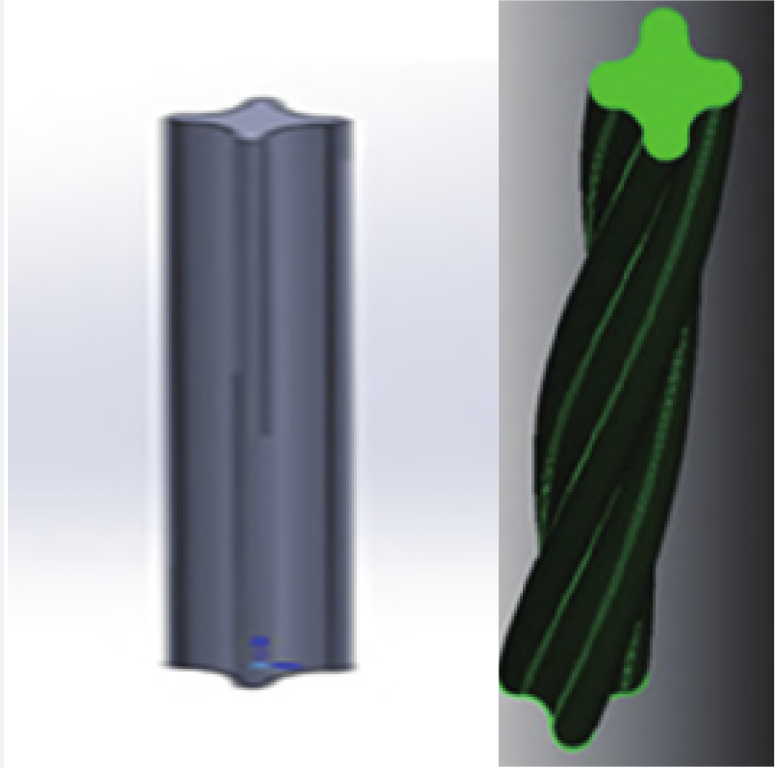
\includegraphics[width=0.4\textwidth]{figures/XiongMinZhiJiYuMengTeQiaLuoJunYunHuaDeYiXingJiHeRanLiaoBangWuLiXingNengYanJiu2023.png}
    \caption{螺旋十字形燃料设计}
    \label{fig:cross_shaped_fuel}
\end{figure}

\section{控制棒的设计及其驱动装置}
控制棒的设计及其驱动装置主要影响中子的控制。对中子的控制主要通过控制棒来实现。控制棒的设计主要包括控制棒的材料、控制棒的驱动装置等。

控制棒一般采用银铟镉(Ag-In-Cd)合金。由于价格低廉、易于加工等特点被广泛应用于压水堆作中子吸收体材料。\cite{ChenHaoHeJiAgInCdHeJinBangCaiLiaoYanJiuJinZhan2019}银铟镉控制棒材料通常密封于不锈钢包壳管中,再和锆合金导向管一起装配成组件,构成压水堆堆芯的控制组件。如图\ref{fig:control_rod}所示。

\begin{figure}[htbp]
    \centering
    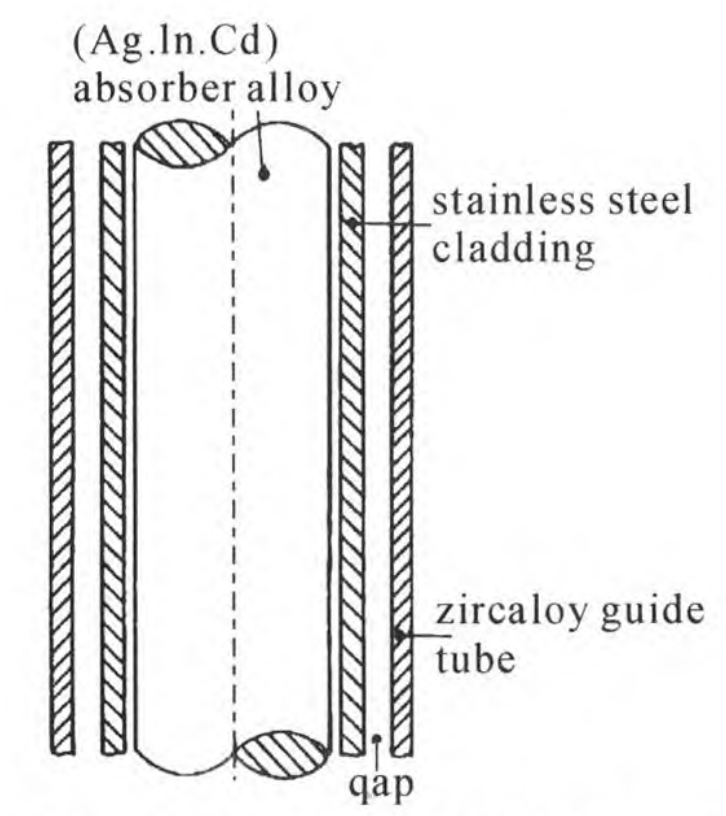
\includegraphics[width=0.4\textwidth]{figures/ChenHaoHeJiAgInCdHeJinBangCaiLiaoYanJiuJinZhan2019.png}
    \caption{Ag-In-Cd合金控制棒}
    \label{fig:control_rod}
\end{figure}

20世纪70年代初开始研发用于替代Ag-In-Cd的控制材料,以应用于当今的反应堆。银占通常使用的Ag-In-Cd材料成分的80\%,已成为一种投机性商品。银和镉的供应也是人们关注的问题,因为这两种材料都被美国政府列为战略材料(出于国家安全考虑),因此可能会供不应求。另一方面,随着锆的全球产量增加,铪的供应在过去十年中有所改善,这使得铪成为一种有吸引力的控制材料。

铪控制杆与之前的Ag-In-Cd控制杆设计基本相同。铪棒取代了每个小杆中的Ag-In-Cd棒,并包含在不锈钢包层内。铪棒和包层之间也留有径向和轴向间隙,以适应控制棒的潜在膨胀。\cite{kellerDevelopmentHafniumComparison1982}
其他的整体控制杆配置、外部尺寸、结构材料以及与反应堆部件和操作设备的接口特性几乎保持不变。

除此之外,由于铪作为反应堆控制材料稀缺且成本高昂,因此人们开发了铪和B的复合控制棒。所开发的制造技术涉及使用锻造铪和3.5 wt\%的Bdispersion钛粉。将两个部件头尾相连,并通过轧制结合技术用钛包裹,该技术使用限制性不锈钢轧制框架来控制两种控制材料在延展性方面的差异。这些复合控制棒已经过弯曲和拉伸测试、热循环、高温水腐蚀测试、控制值以及材料抗辐照损伤性能方面的信息收集。评估研究取得了良好的结果。\cite{cunninghamDevelopmentCompositeControl1958}

对于驱动装置,目前存在水压驱动装置。控制棒水压驱动系统由循环泵、过滤器、组合阀和驱动机构组成。如图\ref{fig:control_rod_drive}所示。反应堆压力容器内的水经循环泵加压后进入组合阀,组合阀有4个出口,其中3个分别与驱动机构的提升水压缸、传递水压缸和夹持水压缸的进水口相连接,另一个与压力容器相连。经组合阀的常闭电磁阀出来的水进入水压缸,靠水的静压驱动水压缸内套向上运动;靠复位弹簧和重力驱动水压缸内套向下运动,排出水压缸内的水经组合阀的常开电磁阀流回压力容器。通过操作组合阀的电磁阀动作,来控制驱动机构中的销爪动作,使驱动轴上下作步进式运动,从而拖动控制棒运动达到控制反应堆的目的。\cite{BoHanLiangHeFanYingDuiKongZhiBangShuiYaQuDongJiShu2005}

\begin{figure}[htbp]
    \centering
    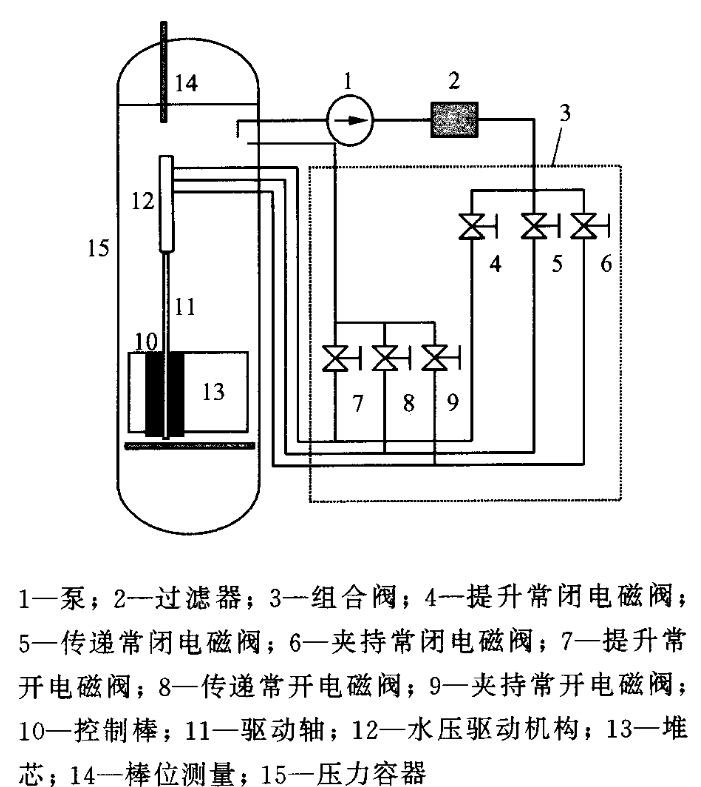
\includegraphics[width=0.4\textwidth]{figures/BoHanLiangHeFanYingDuiKongZhiBangShuiYaQuDongJiShu2005.png}
    \caption{控制棒驱动装置}
    \label{fig:control_rod_drive}
\end{figure}

\bibliography{cite.bib}

\vspace{3em}

{
    \centering\textbf{\huge Neutron Generation, Transport and Control in Pressure Vessel}\\
}

\section*{Abstract}

This article provides an overview of neutron generation, transport and control mechanisms in pressurized water reactors, as well as design approaches for core fuel and control rods. In pressurized water reactors (PWRs), neutrons are mainly produced by fission of uranium-235 or plutonium-239, and the energy is continuously released through a chain reaction. The neutron transport is determined by the collision of neutrons with the medium and can be described by the neutron transport equation. Reactive control methods include control rods, combustible poisons, and boric acid. These methods modulate reactor reactivity by varying neutron absorption, moderating capacity, or fuel content, and are generally used in combination in pressurized water reactors to reduce the number of control rods. Core fuel design involves factors such as fuel material, shape, and arrangement. Optimizing the fuel loading configuration can improve energy output and reactor safety. Control rod design focuses on material selection, mainly silver-indium-cadmium or hafnium alloys, improved by composite materials and equipped with hydrodynamic drive systems to achieve effective control.

\subsubsection*{Keywords: 1. Pressurized Water Reactor, 2. Nuclear Reactor, 3. Core, 4. Nuclear Energy, 5. Thermal Hydraulics}

\end{document}